\section{Introduction}
\subsection*{Project Idea}
Occasionally people will wonder about what is happening in the neighborhood where they reside and wether or not it is still safe.
We found a solution to this problem. 
We created a program in which people can search for their (home)city to see what is happening. 
They will receive a news feed of articles concerning their neighborhood and a list (visualized by circles on a map) of events in which the emergency services were involved. 
To retrieve these, we will use the P2000 system used in the Netherlands. The news feed will either be extracted from local news sites and Twitter.

\subsection*{Data}
The data that we will use for our project will be extracted from several different sources. 
These sources can be cut in two clear distinct parts. 
One part consists of data that we will extract out of the P2000 system used in the Netherlands. 
This system contains notifications of events which involved emergency services. 
There are several sites which can be used to retrieve this data.
The second part contains the news feed and Twitter data we want to show when people are searching for their city. 
The Twitter data comes from Twitter itself, the local news will be retrieved from several local news sites. 

\subsection*{Achieved Goals}
We achieved almost all the goals we had set for our self in this project. 
What we wanted to create was a system where people can search for a city and a time frame.
When they do, we want to visualize a map of the Netherlands zoomed in on that city. 
The map will contain several colored dots. 
Every dot will represent an event in which the emergency services were involved. 
We want to use different colors for different services (police, fire department and ambulance) and let the size of the circle depend on how serious the event was. This is the basic outline of the project which has to work for 100$\%$. Furthermore, we want to be able to click on the circles which will trigger a pop up to appear with local, related news to the event. This news is extracted from either Twitter or local news sites as mentioned before. Another feature we would like to implement is to use classifications in the search. For example I would like to only see events which involved murder or robbery. We do not know how difficult this will turn out to be, so we regard this as an optional feature.\\
The realized project does something quite similar, we are able to search for a city and that city is visualized on a map.
P2000 notifications are now represented with pins on a map. 
The color of the pin represents whether a notification concerns the police (blue), the fire fighters (red) or an ambulance (yellow).
When a person selects a notification on the right-hand side related news and twitter is shown.\\
The things that we did not achieve to do is to do this real-time or for the whole country. 
For doing this real time, it just takes too long to crawl the news sites and notifications and to index all the retrieved data.
We were able to do this for a test set of data consisting a week and several locations.\\
Also the associations we wanted to create the between the notification and twitter and news was not as strong as we wanted it to be.
This is due to the fact that it turned out to be very difficult to relate every notification to twitter feed and news about that event (if there was such data).
Therefore we settled that we want to show related news to the notification.
For example if you click on a fire notification, we show news about other (or possibly the same) fires in the neighborhood.
This type of association was easier to create.\\
The eventual code for the whole project can be found \href{https://www.dropbox.com/home/Public/Code_2IMW15_Group_20}{here}.

\begin{center}
\begin{figure}[h!]
  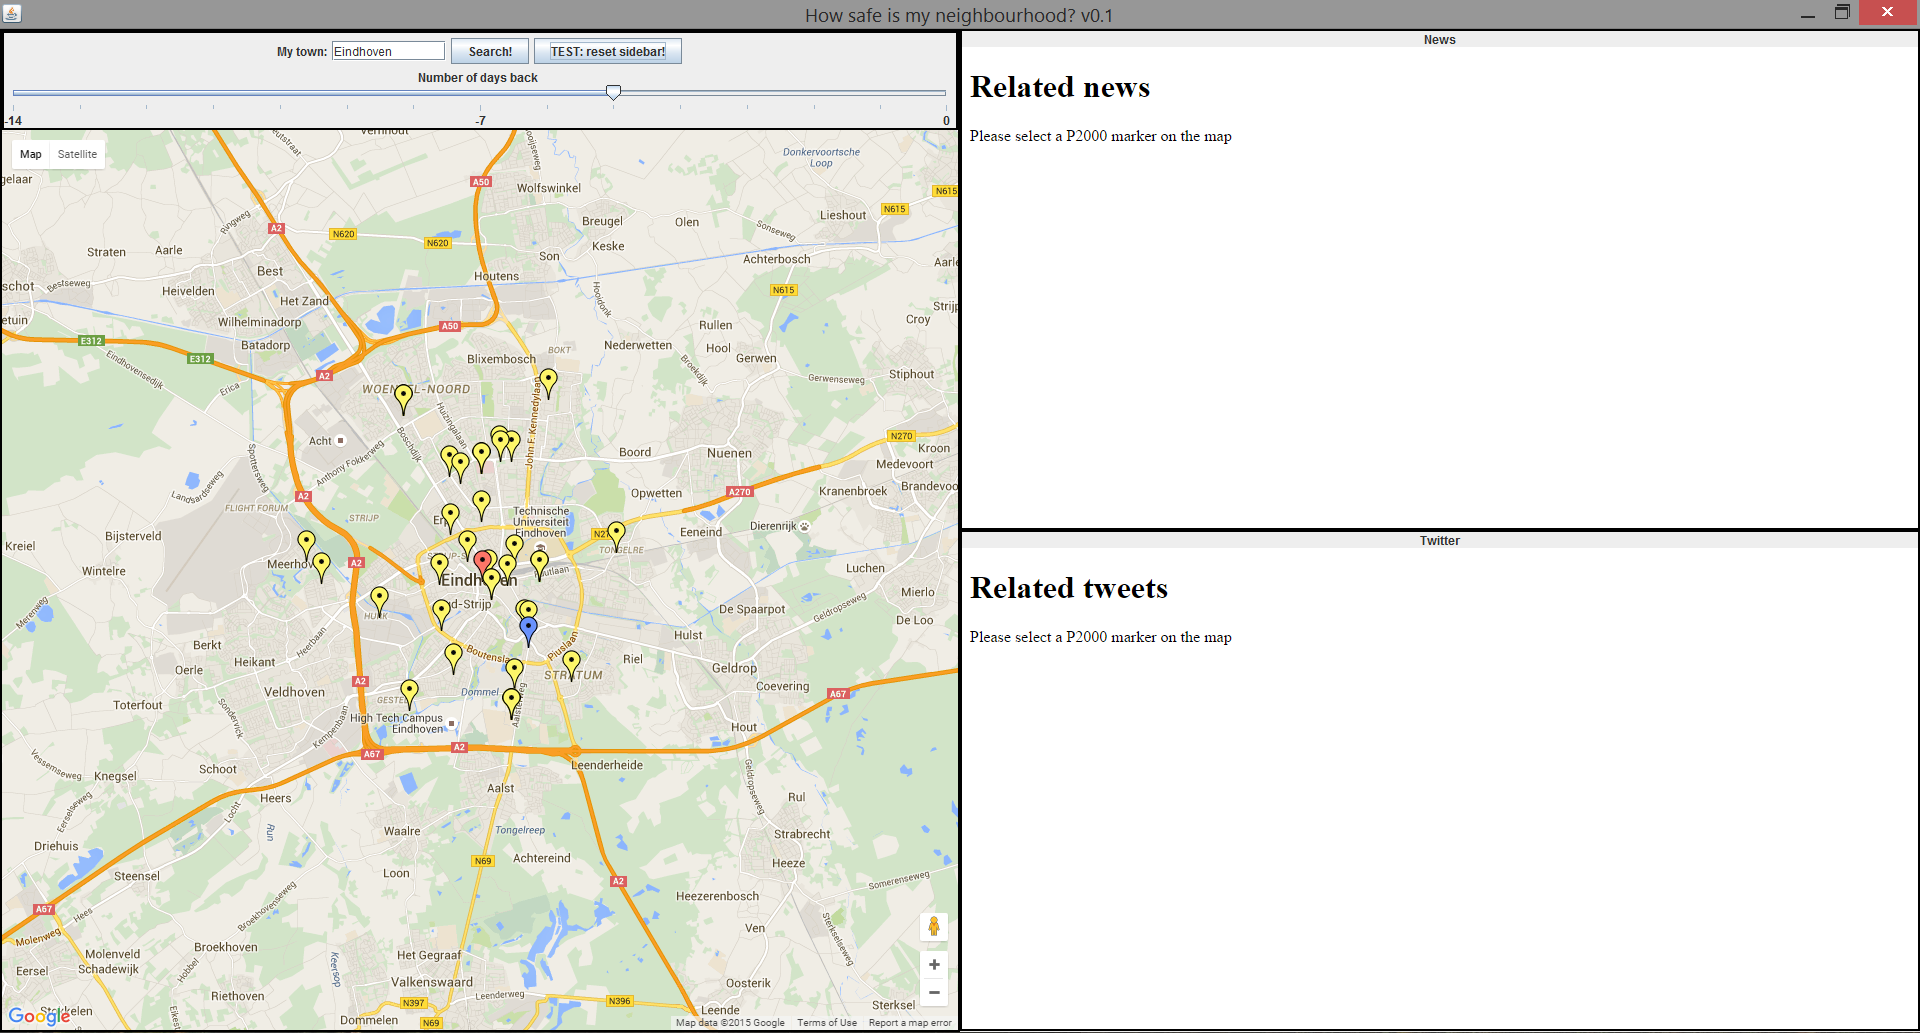
\includegraphics[width=0.85\textwidth]{GUI-colours.png}
  \caption{Graphical User Interface showing different types of P2000 notifications}
  \label{fig:GUI-colours}
\end{figure}

\begin{figure}[h!]
  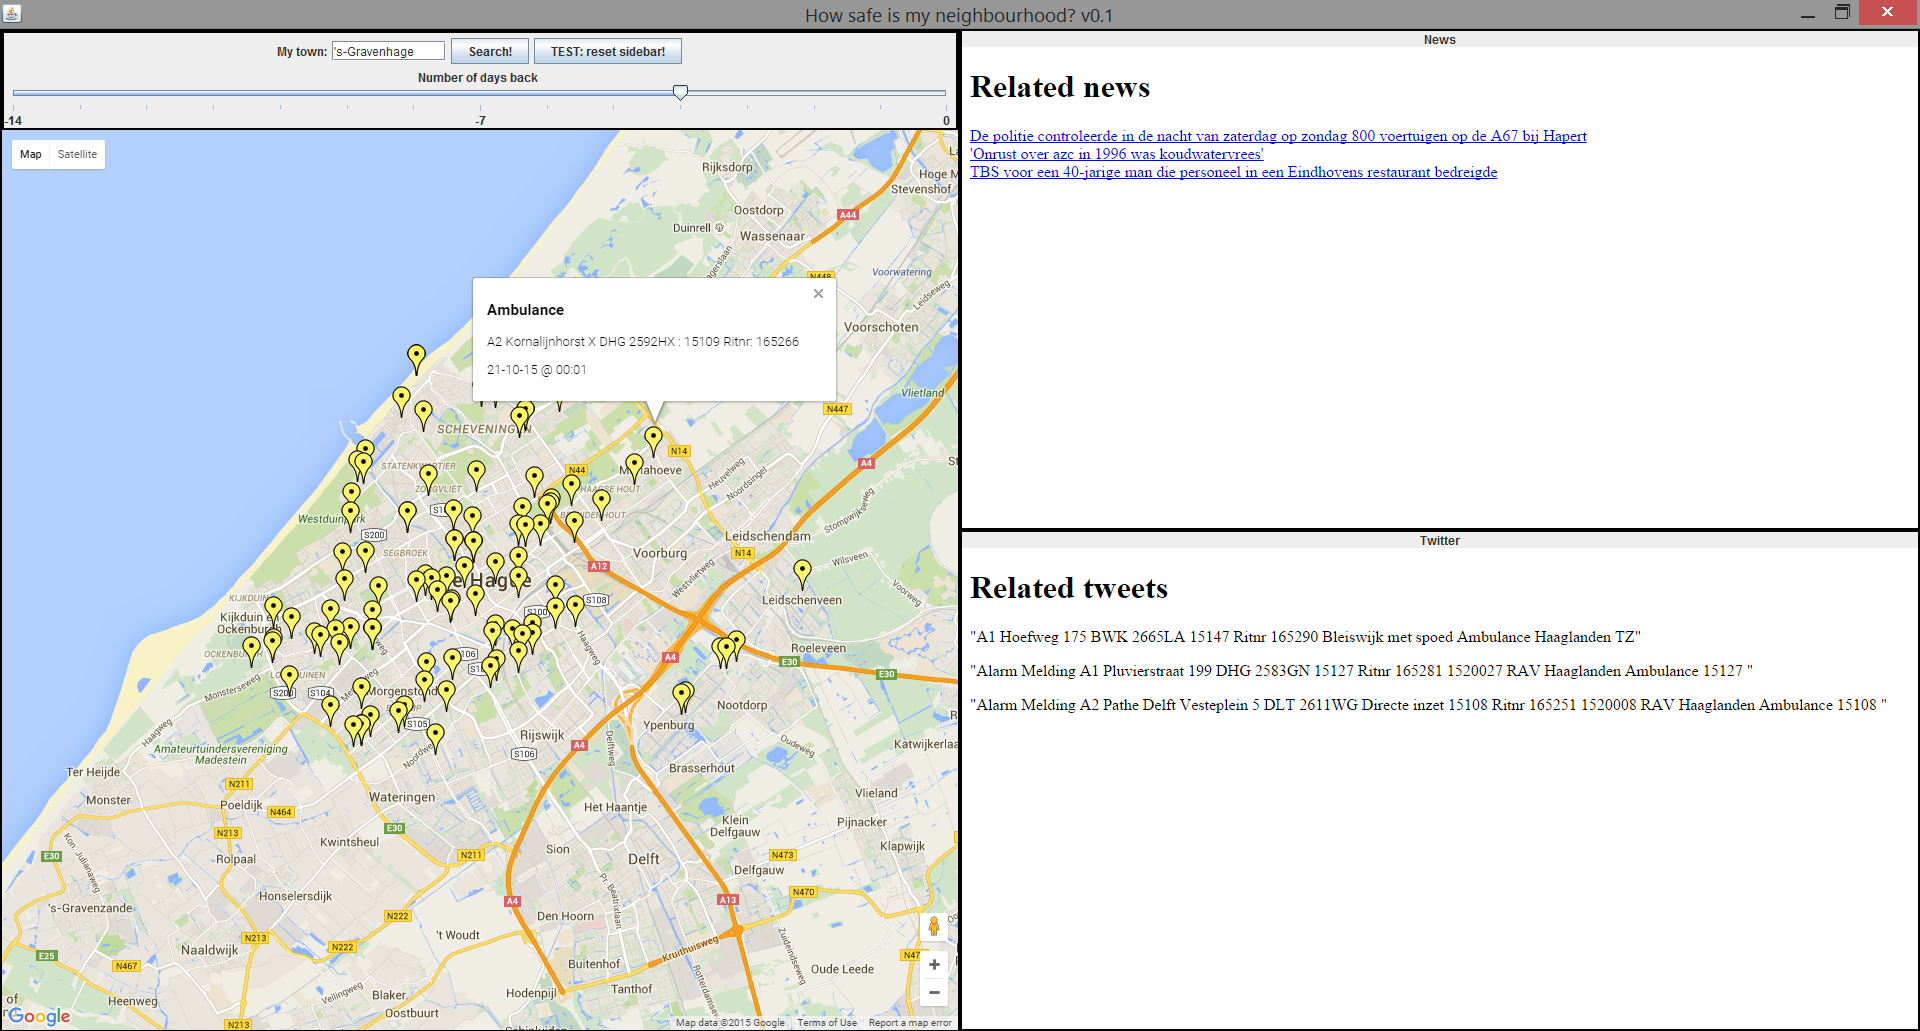
\includegraphics[width=0.85\textwidth]{GUI-newsandtwitter.png}
  \caption{Graphical User Interface showing related news and tweets}
  \label{fig:GUI-newsandtwitter}
\end{figure}
\end{center}

\subsection*{Tasks}
The IR and ML tasks are divided such that one person contributes at at least one of each. The tasks are shown in \autoref{tab:tasks}

\begin{table}[!h]
\begin{center}
\begin{tabular}{|l|l|l|l|}
\hline
            		& {\bf Student ID} 	& {\bf Information Retrieval}                                                                                      						& {\bf Machine Learning} \\ \hline
Francis Hoogendijk 	& 0834628          	& Collect P2000 Notifications                                                                                     						& \begin{tabular}[c]{@{}l@{}}Classify Twitter Data \\ $\&$ Create GUI\end{tabular} \\ \hline
Bram Kohl          	& 0746107          	& Indexing of Notifications                                                                                        						& Cluster Notifications \\ \hline
Guus van Lankveld  & 0629468          	& Collect News Feed                                                                                                						& \begin{tabular}[c]{@{}l@{}}Association Analyzer \\ Between P2000 \\  Notifications $\&$ News\end{tabular} \\ \hline
Jasper Selman      	& 0741516          	& \begin{tabular}[c]{@{}l@{}}Language Detection \& \\ Spell Check\end{tabular}         					& \begin{tabular}[c]{@{}l@{}}Classify News Feed\end{tabular}            \\ \hline
Ramon de Vaan      	& 0758873          	& \begin{tabular}[c]{@{}l@{}}Create Database of P2000 \\ Notification Codes \& \\ Collect Twitter Data \end{tabular}  	& \begin{tabular}[c]{@{}l@{}}Association Analyzer \\ Between P2000 \\  Notifications \& Twitter\end{tabular}  \\  \hline
Bart van Wezel     	& 0740608          	& \begin{tabular}[c]{@{}l@{}}Indexing of News Feed / \\ Twitter Data\end{tabular}                                  			& Classify P2000 Notifications \\ \hline
\end{tabular}
\caption{Tasks}
\label{tab:tasks}
\end{center}
\end{table} 